\documentclass[10pt]{article}
\usepackage[margin=.78in]{geometry}
\usepackage[T1]{fontenc}
\usepackage{lmodern,microtype,booktabs,tabularx,graphicx,hyperref,xcolor}
\emergencystretch=3em
\title{External Cohort Evaluation of IDM-Viz\\UCI Gas Sensor Array Drift Dataset}
\author{Umar Behram (23I-2604) \and Ahmed Bilal (23I-2581)}
\date{Day 2 research extension -- 15 November 2026}
\begin{document}
\maketitle
\begin{abstract}
We evaluated a frozen multiclass logistic model and the IDM-Viz input/impact channels on the UCI Gas Sensor Array Drift dataset (UCI 224). The source contains 13,910 rows, 128 numeric features, six gas classes, and ten acquisition batches. Batch 1 alone supplied a locked stratified training/calibration/reference split; whole batches 2-10 were held out. Across those nine cohorts, mean accuracy was 0.432 and fixed-six-class macro-F1 was 0.290. The calibrated confidence estimate averaged 0.976, with mean absolute accuracy-estimation error 0.545. Its approximate 95% plug-in intervals covered 0/9 cohort accuracies. The result is a pronounced calibration-transfer failure on this dataset under a small historical split, not evidence of general performance or independent replications.
\end{abstract}

\section{Provenance and admission}
The source is UCI dataset 224 \cite{uci224}. Its archive SHA-256 is in \path{docs/phase3/research_improvement_day2/SOURCE_HASHES.sha256}. Source-only inspection confirmed ten batch files, 13,910 rows, 128 finite feature values per row, all six classes in batch 1, and no exact duplicate records across the archive. Batch sizes range from 161 to 3,613 except batch 1 (445); class coverage varies and some cohorts omit class 6. The UCI page reports CC BY 4.0 while its dataset description also says research use only and excludes commercial purposes. We honor the more restrictive research-only statement. Acquisition batch order is coarse; original files provide no within-cohort event timestamps. We do not invent timestamps or exact drift-onset labels.

\section{Locked protocol}
Before fitting or inspecting monitoring outcomes, we locked a 60/20/20 stratified split within batch 1 using fixed seeds 2242026 and 2242027. This yields 267 training, 89 calibration, and 89 reference rows. A first implementation mistakenly allocated 134/133/178; those initial results remain preserved under a separate v1 results path and are excluded here. The corrected run uses only the locked partition. The small historical sample is a material limitation. The frozen model is standardized multinomial logistic regression (C=1); scaler, PCA, and model fit on training rows only. A fixed logistic mapping from maximum class probability to correctness is fit on calibration rows only. Decisions use argmax model probability. No batch 2-10 outcome is used for fitting, threshold selection, or protocol choices.

Each whole future batch is a cohort. Input evidence uses two-sided KS tests on 128 features and three frozen PCA scores, Holm-adjusted within cohort at 0.05. Impact is average calibrated correctness with a continuity-corrected normal approximation to a plug-in Poisson-binomial predictive interval. This interval assumes independent Bernoulli correctness probabilities and omits calibration uncertainty; it is not a confidence interval for population accuracy. Historical accuracy and raw mean maximum probability are baselines. We report accuracy, macro-F1 over fixed labels 1-6, per-class precision/recall/F1/support, estimation error, interval coverage/width, class composition, and alarm burden.

\section{Results}
Across batches 2-10, the average accuracy was 0.432, macro-F1 0.290, estimated accuracy 0.976, and estimation MAE 0.545. All nine cohorts triggered at least one Holm-adjusted input test; this is an alarm burden of 9/9 cohorts, not known-onset recall. The approximate interval missed all nine observed cohort accuracies, with mean width 0.026. Since there is one ordered dataset and nine heterogeneous cohorts, coverage is a descriptive tally, not an inferential estimate.

\begin{table}[h]
\centering\small
\begin{tabular}{rrrrrrr}
\toprule Batch & n & Accuracy & Macro-F1 & Estimated & Abs. error & Tests rejected\\
\midrule
2 & 1244 & .603 & .522 & .975 & .373 & 109/131\\
3 & 1586 & .623 & .392 & .976 & .354 & 124/131\\
4 & 161 & .658 & .347 & .977 & .318 & 110/131\\
5 & 197 & .320 & .247 & .976 & .657 & 111/131\\
6 & 2300 & .449 & .234 & .977 & .528 & 121/131\\
7 & 3613 & .387 & .290 & .976 & .589 & 102/131\\
8 & 294 & .194 & .166 & .975 & .781 & 131/131\\
9 & 470 & .343 & .186 & .976 & .633 & 126/131\\
10 & 3600 & .307 & .226 & .976 & .669 & 70/131\\
\bottomrule
\end{tabular}
\caption{Whole-batch evaluation. Fixed six-class macro-F1 assigns zero score to a class absent from a cohort; use supports in the companion per-class CSV.}
\end{table}

\begin{figure}[h]
\centering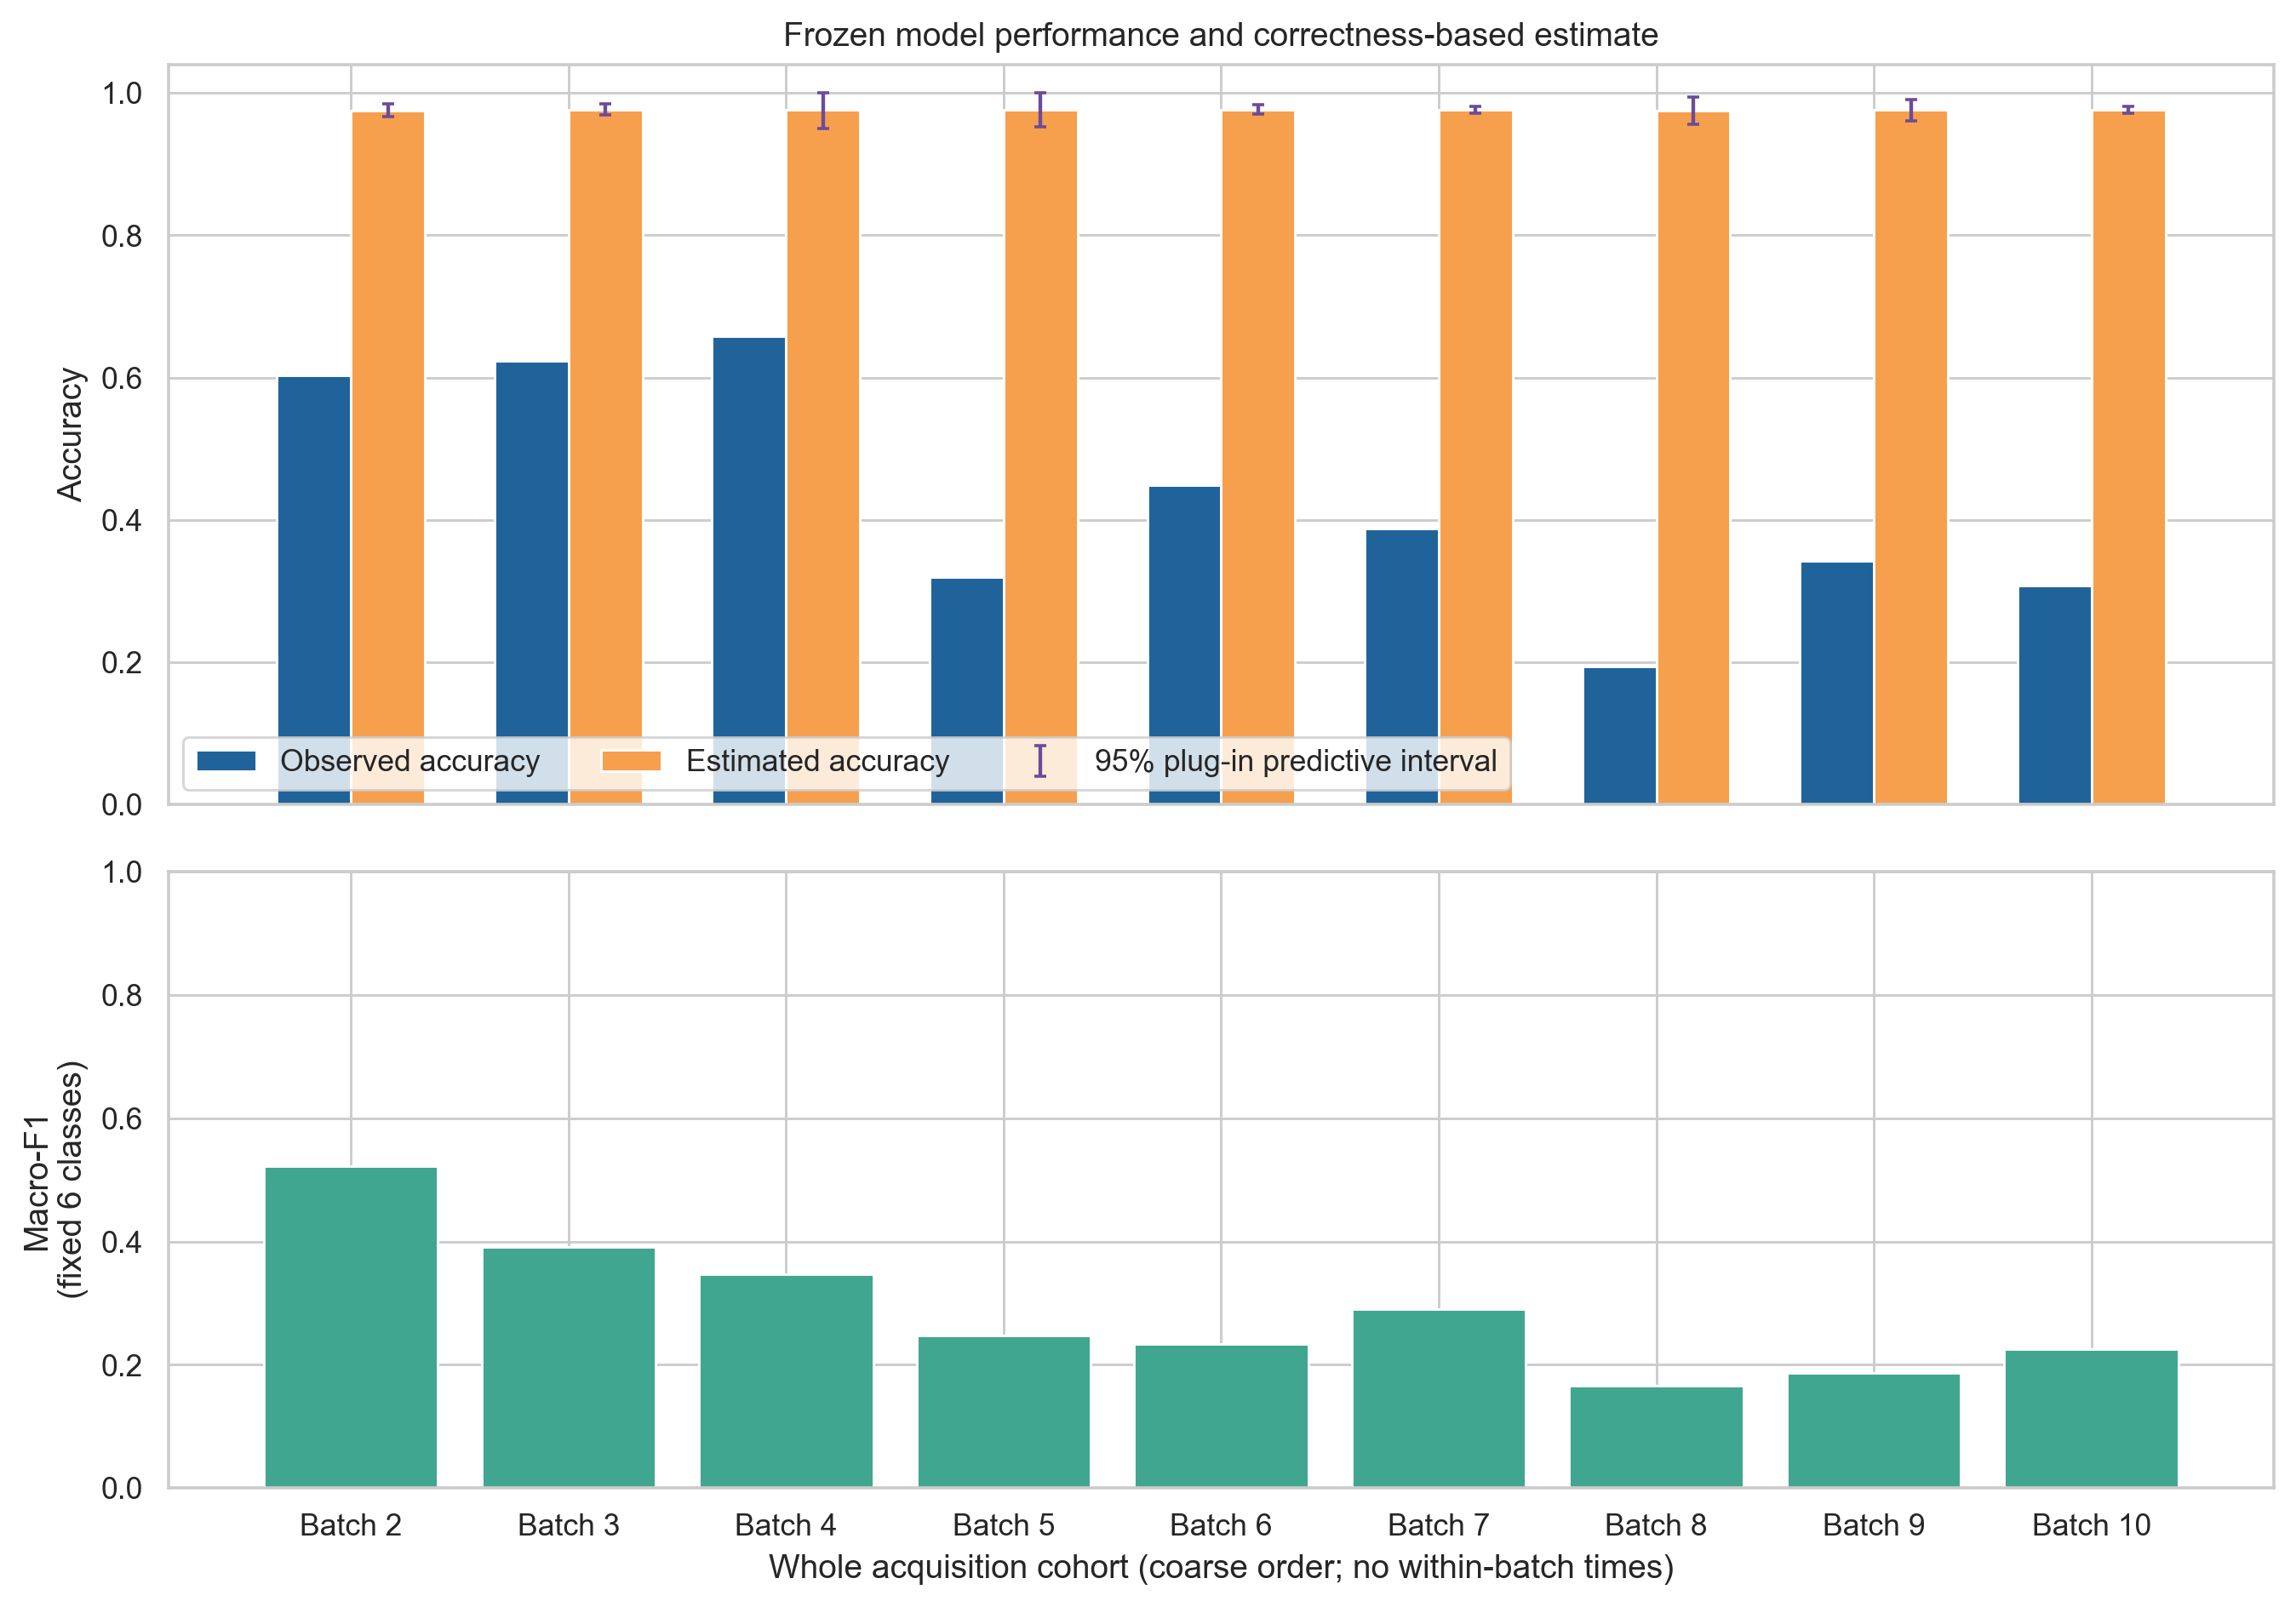
\includegraphics[width=.93\linewidth]{figures/cohort_performance.png}
\caption{Observed and estimated performance by held-out cohort; estimated intervals are approximate plug-in prediction intervals.}
\end{figure}

\begin{figure}[h]
\centering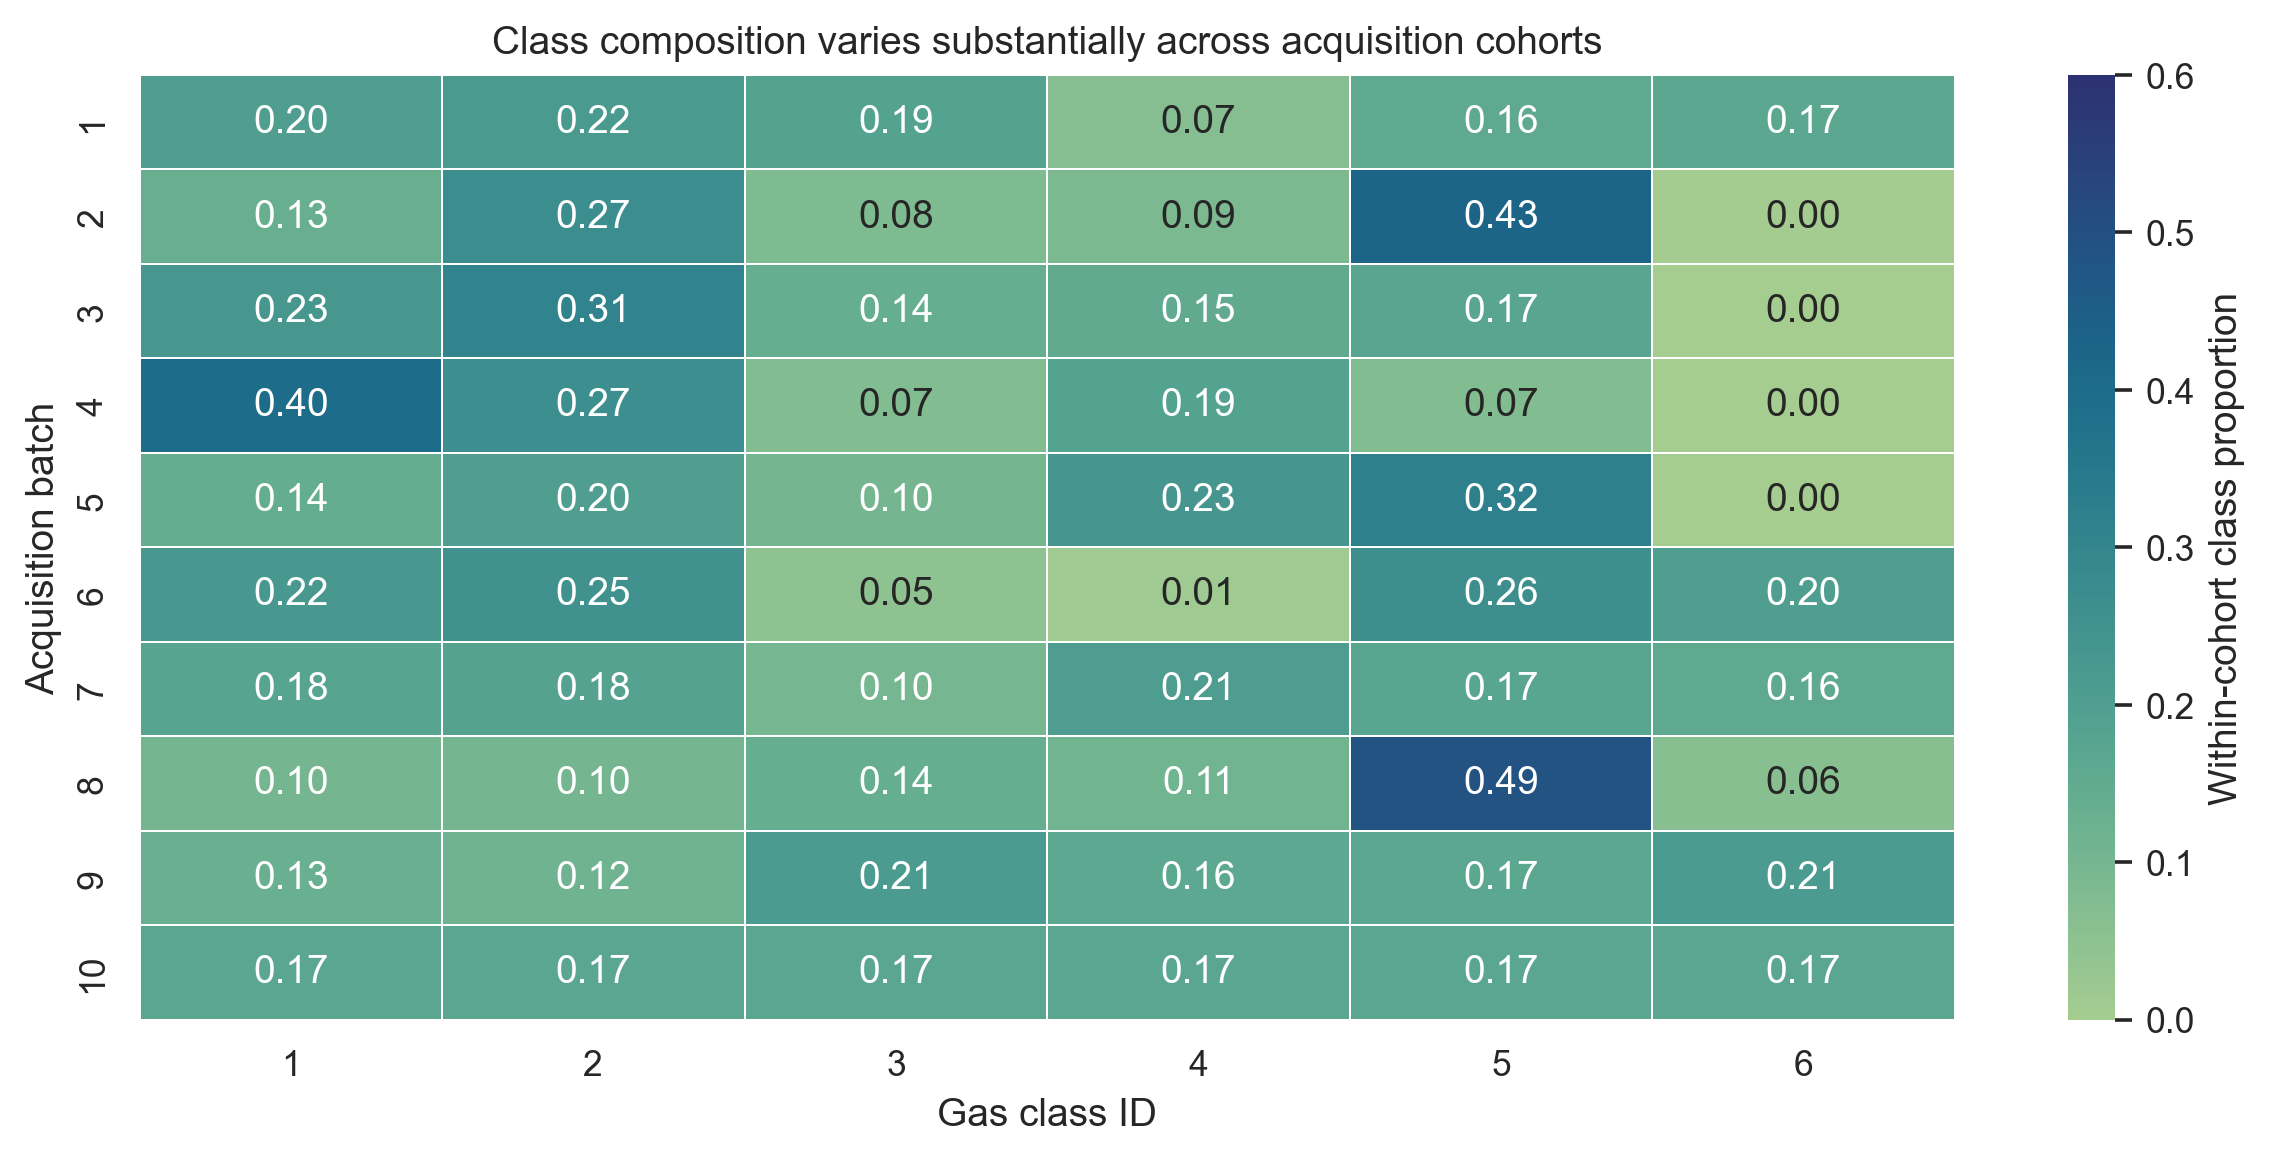
\includegraphics[width=.83\linewidth]{figures/class_composition.png}
\caption{Observed class proportions vary by acquisition batch, affecting aggregate accuracy interpretation.}
\end{figure}

\section{Interpretation and limitations}
Input alarms indicate detectable feature-distribution differences, but do not identify harm. The confidence estimate remains near .985 despite accuracy as low as .133. The 134-row calibration sample had accuracy 132/134; the 178-row reference had 173/178. This makes the external result a strong warning about calibration transfer, but its magnitude is conditioned on a small, single-batch history. Class proportions differ substantially across later cohorts, and per-class results show heterogeneous degradation. No causal attribution to class mix or time is claimed. Batch-level order is not fine-grained chronology, cohort sizes are unequal, and absent classes make some per-class metrics undefined. This is one external dataset, not independent replication or known-onset drift recall.

The external extension changes the original binary synthetic setup to multiclass cohort evaluation; it does not reproduce delayed online label release. The Phase 2 DOCX remains the methodological basis, and Phase 2 received no instructor feedback. Implementation choices and deviations are recorded in the locked protocol and source notes. The study used local CPU; execution and reproduction commands are in \path{docs/phase3/research_improvement_day2/README.md}.

\bibliographystyle{plain}
\bibliography{REFERENCES}
\end{document}
